\documentclass[12pt]{article}
\usepackage[margin=1.0in]{geometry}
\usepackage{graphicx}
\usepackage[pdftex]{hyperref}
\usepackage{wrapfig}
\usepackage{float}
\usepackage{enumitem}
\usepackage{textcomp}
\usepackage[english]{babel}
\usepackage{csquotes}
\usepackage[document]{ragged2e}
\usepackage[utf8]{inputenc}
\usepackage{indentfirst}
\usepackage{nicefrac}

\MakeOuterQuote{"}
\renewcommand{\baselinestretch}{1.15}
\setlength\parindent{0.5in}
\setlength\RaggedRightParindent{\parindent}
\setlength\parskip{1em}
\let\supscr=\textsuperscript


\begin{document}
\begin{titlepage}
    \centering
    \vspace{15cm}
    {\huge\bfseries Subsystems Report \par}
    \vspace{1cm}
    {\scshape\Large Jonathan Sumner Evans\par}
    \vfill
    {\scshape\large Section U\par}
    {\large \today\par}
    \vfill
\end{titlepage}

\section{Introduction}
A food desert is an area where access to fruits and vegetables is limited, too expensive, or
nonexistent due to a lack of grocery stores and farmers markets within a convenient walking
distance \cite{cdc-food-deserts}. People living in food deserts often rely on fringe food retailers
and discount stores, such as gas stations and dollar stores, for food. These retailers tend to sell
high-fat and processed foods which contributes to higher rates of obesity and diabetes in those food
desert areas. According to the US Department of Agriculture, there is a food desert in the Wheat
Ridge area located between Wadsworth, 32\supscr{nd} Avenue, and 38\supscr{th} Avenue
\cite{usda-food-deserts}.

The team’s goal is to empower English and Spanish speaking Wheat Ridge residents over 65 years in
age who live in a food desert and rely on food stamps to utilize a self-sustaining plant growing
system. Most of the system will come prepackaged for safe installation and use and will partially
use materials that can be sourced in the Wheat Ridge neighborhood. The net cost will be neutral or
better after two years of plant harvest and will include features that consider the potential
physical limitations of the stakeholders.

\section{Solution Description}
The team’s design addresses the problem with a system composed of five distinct and interconnected
subsystems. The structural subsystem involves a three-tiered structure that is compact, lightweight,
and cost-effective, so that the stakeholder can easily install and maintain it. With it’s 12 hole
design and the reservoir at it’s base, the structure is the key connection between the hydroponic
soda bottle system and the watering system. Furthermore,  the watering system consists of two
symbiotic subsystems: the reservoir and the cascading water system.  The reservoir system uses four
separate water tanks, which correspond to each growing stage in the plant cycle. The water is
delivered to each plant by pumping water to the bottles in the top tier of the structure; the water
then cascades down to the next two rows through tubing that connects the bottles together and
finally returns back to the reservoir. This system only requires the stakeholder to refill the
reservoirs one time per week. The nutrient subsystem is housed partially within the reservoir.
Along with the structure and watering system, the stakeholder will receive packages of pre-measured
nutrients that correspond to the growing cycle of the plants. Using a color-coding system, the
stakeholder simply has to fill the reservoirs with the nutrients and water, which will then be
delivered to the plants via the water delivery system. Finally, the hydroponic (soilless) soda
bottle system is composed of re-purposed 2-liter soda bottles and materials that can easily be
sourced in the Wheat Ridge food desert. The soda bottles are the foundation for the snow peas,
lettuce, and spinach to grow. The water-nutrient mixture is pumped into the bottles and is carried
to the plant via a wick. This design prevents the stakeholder from overwatering and underwatering
the plants and lowers the cost of the entire system by using easily-sourced substrate in lieu of
soil. The final solution also includes a tool which will allow the stakeholders to easily construct
the bottle systems themselves despite their physical limitations. These five interconnected
subsystems comprise our final solution: an elegant, easy-to-maintain food growing system designed
with the stakeholders’ needs in mind.

\section{Subsystem Description}

% - Describe your subsystem functionality and key components.
% - Physical properties, including dimensions, material type, specifications, weight, and
%   construction.
%       - Include sketches with dimensions instead of long physical descriptions.

The water delivery subsystem transports water from the reservoirs to the top set of bottles and from
the top bottles to the lower bottles. The three major components of the water delivery are as
follows:

\begin{enumerate}
    \item \textbf{Reservoir Ceiling Connection:} The water must be pumped out of the reservoir
        through the ceiling of the reservoir. This connection point is the boundary of the water
        delivery subsystem. The connection at this interface point must be watertight.

    \item \textbf{Tubing:} From the reservoir ceiling, $\nicefrac{1}{2}"$ tubing will carry the
        water to the top bottle. Light causes nutrients to decompose, thus this tubing will be black
        to reduce the water's exposure to light.

    \item \textbf{Connections to Bottles:} The tubing connects to the bottles at two points: the top
        entry and the drain exit.

\end{enumerate}

\section{Subsystem Interfaces}

% - Explain the interfaces with the other subsystems: describe each interface and how your design
%   addresses each. Reference a figure or a table.

% - Reservoir Ceiling
The water must be pumped out of the reservoir through the ceiling of the reservoir. This connection
point is the boundary of the water delivery subsystem. The connection at this interface point must
be watertight.


% - Bottle connection



\section{Subsystem Analysis}

% - Validation that it will work. If tested, what was the design of your experiment/test, and what
%   was the result?  If not tested, prove through research and analysis that your concept will
%   function as planned.

\section{Summary}

% - Given your research, stakeholder feedback and/or testing, what are your recommendations for
%   design iterations and design implementation into the final, full-scale, production solution?

\pagebreak
%\begin{figure}[H]
%    \centering
%    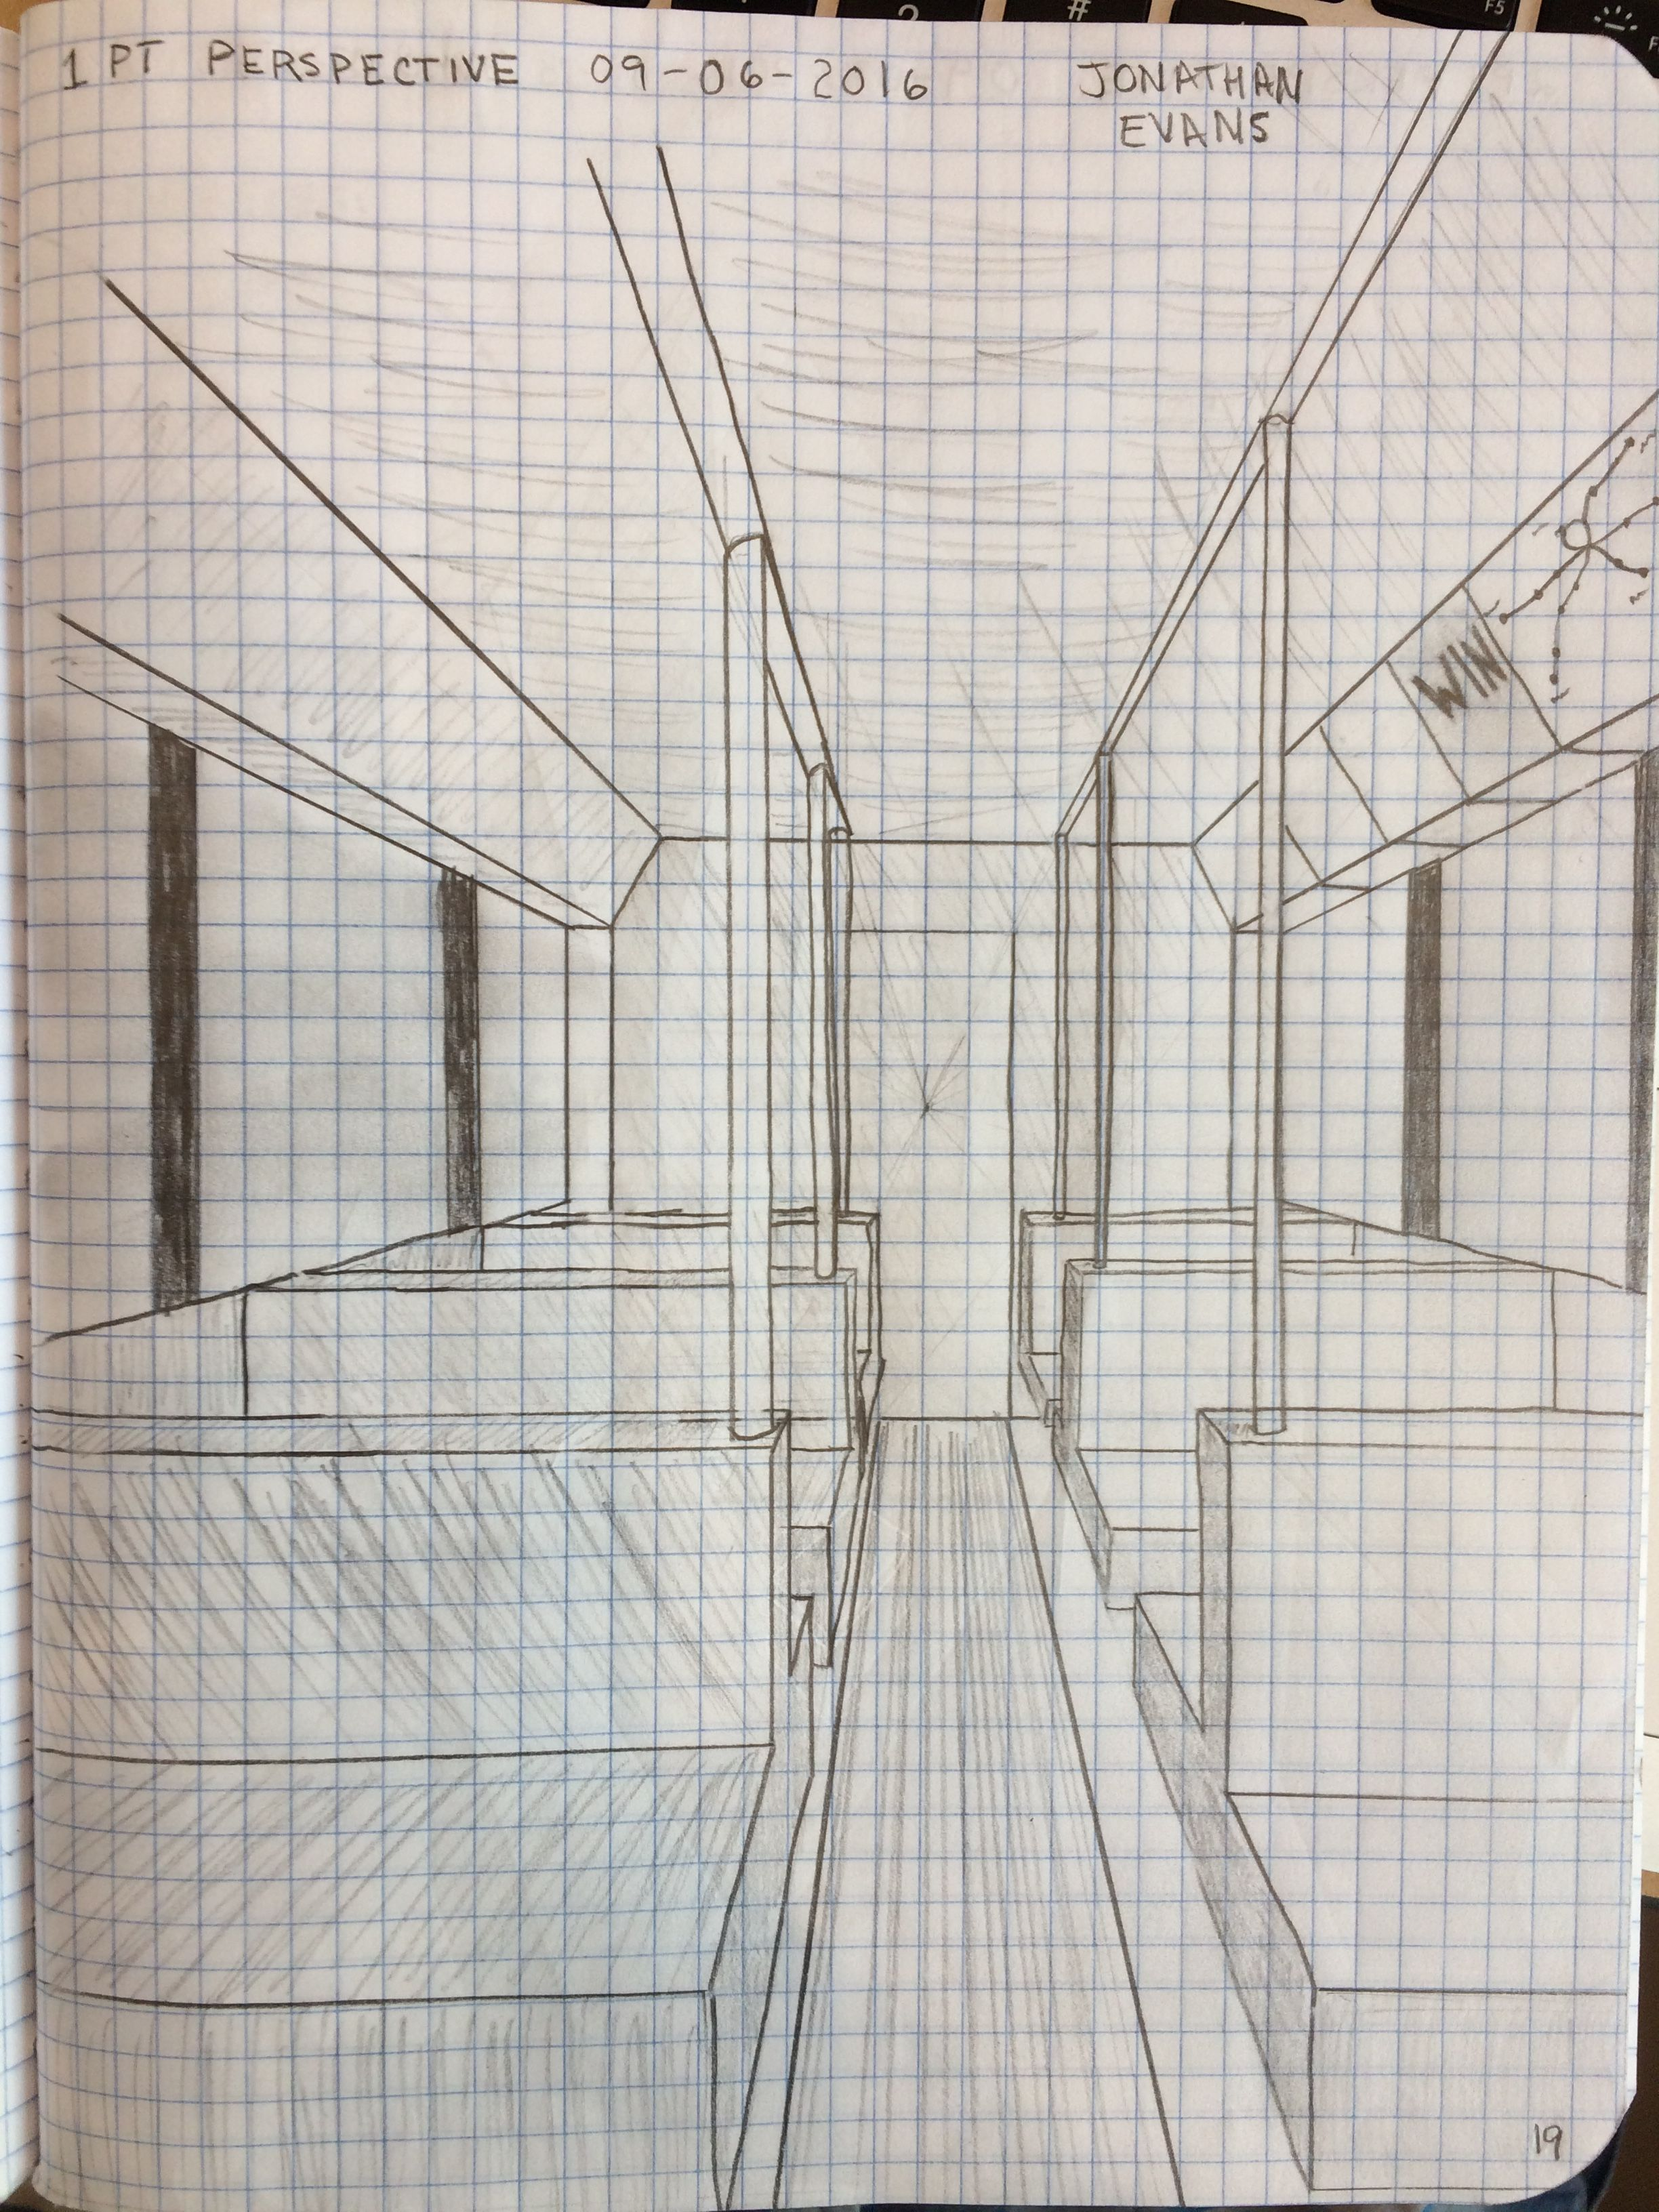
\includegraphics[width=160mm]{resources/light-rail-sketch.jpg}
%    \caption{Sketch of Inside of Light Rail}
%\end{figure}

\pagebreak

\begin{thebibliography}{9}
    \bibitem{cdc-food-deserts}
    Centers for Disease Control and Prevention (2012).
    \textit{A Look Inside Food Deserts} [Online].
    Available: \url{http://www.cdc.gov/features/FoodDeserts/index.html}.
    [Accessed 11 Sept. 2016].

    \bibitem{usda-food-deserts}
    United States Department of Agriculture Economic Research Service (19 Oct. 2016).
    \textit{Food Access Research Atlas} [Online].
    Available:
    \url{http://www.ers.usda.gov/data-products/food-access-research-atlas/go-to-the-atlas.aspx}.
    [Accessed: 28 Oct. 2016].

\end{thebibliography}

\end{document}
